\section{Experiments}
\label{sec:evalution}

We evaluate our method both quantitatively and qualitatively on text-guided editing of real images. We analyze the usage of our extracted latent code by itself (as explained in Sec.~\ref{sec:text-guided}), and in combination with existing methods that currently use DDIM inversion. In the latter case, we extract the noise maps using our DDPM-inversion and inject them in the reverse process, in addition to any manipulation they perform on \eg attention maps. All experiments use a real input image as well as source and target text prompts.% Similarly to~\cite{Hertz22,Wu22,Gihyun22,Kim22}, our method needs also an initial prompt. 
% However, as shown in Parmar et al.~\cite{Parmar23}, it can be generated using an image captioning network. 


% we use the popular and publicly available Stable
% Diffusion model~\cite{Rombach22} where the diffusion forward process is applied on a latent image encoding and an image decoder is employed at the end of the diffusion backward process.


\vspace{-0.3cm}
\paragraph{Implementation details} We use Stable Diffusion~\cite{Rombach22}, in which the diffusion process is applied in the latent space of a pre-trained image autoencoder. The image size is $512\! \times 512 \!\times \!3$, and the latent space is $64 \! \times 64 \! \times \! 4$. Our method is also applicable in unconditional pixel space models using CLIP guidance, however we found Stable Diffusion to lead to better results. 
% , unless noted otherwise
Two hyper-parameters control the balance between faithfulness to the input image and adherence to the target prompt: the strength of the classifier-free guidance~\cite{Ho21}, and $T_{\text{skip}}$ explained in Sec.~\ref{sec:text-guided}. In all our numerical analyses and all the results in the paper, we used $\text{strength}\!=\!15$,  $T_{\text{skip}}\!=\!36$, $\eta\!=\!1$ and $100$ inference steps,  unless noted otherwise. 
In the SM we provide a thorough analysis of the effect of the strength and $T_{\text{skip}}$ hyper-parameters.


\begin{figure}[h]
\centering
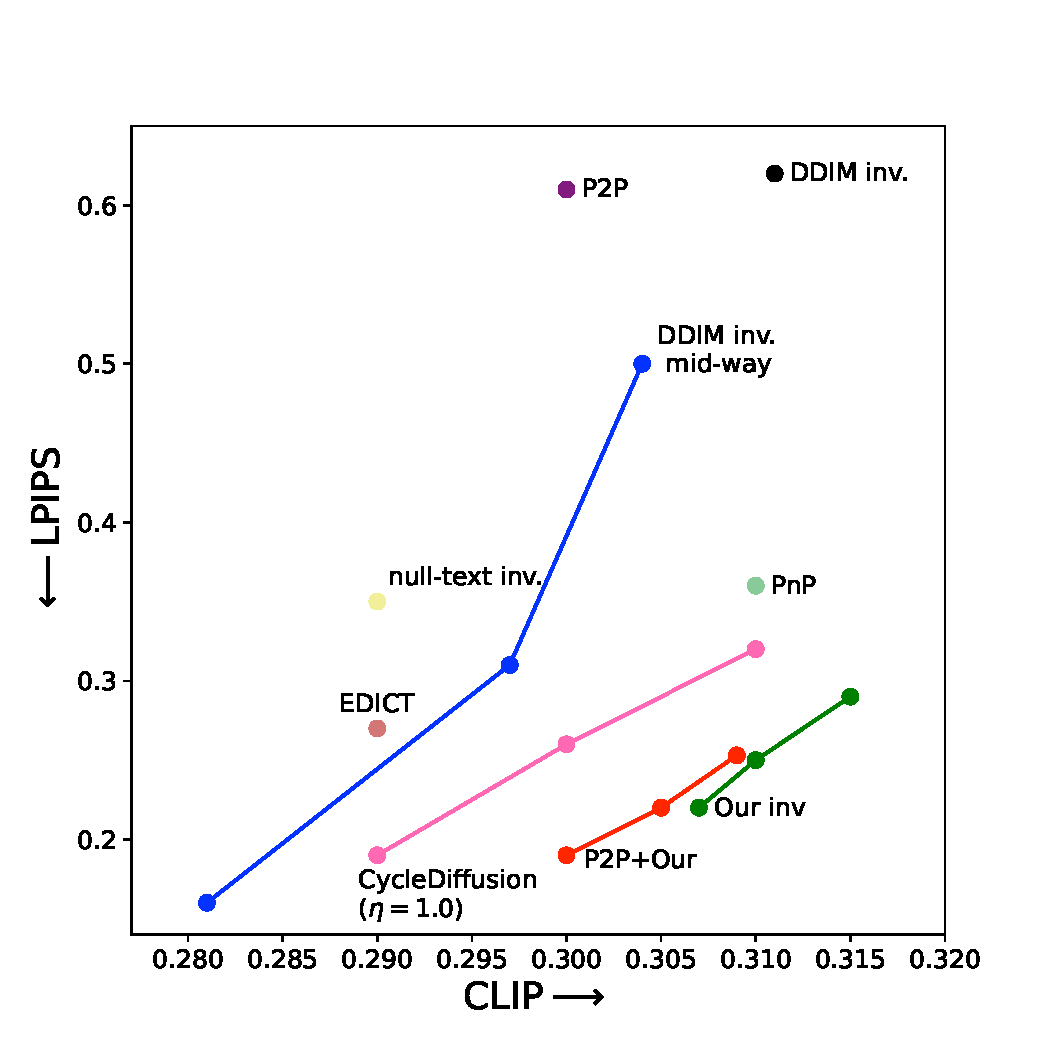
\includegraphics[trim={0 0.7cm 0 2.1cm},clip=true,width=1\columnwidth]{ICCV23_submission/figures/clip_lpips.pdf}
\caption{\textbf{Fidelity to source image vs.~compliance with target text.} The plot compares the LPIPS and CLIP scores achieved by all methods on the modified ImageNet-R-TI2I dataset.  Our inversion, P2P with our inversion, and CycleDiffusion are shown with three options of the parameters (strength,$T_{\text{skip}}$): for our method $(15,36),(12,36),(9,36)$, for P2P+Ours $(7.5,8),(7.5,12),(9,20)$, and for CycleDiffusion $(3,30),(4,25),(4,15)$. DDIM inversion mid-way is shown with three options for $T_{\text{skip}}$: $20, 40, 60$, all with a guidance strength of 9. The parameters for the other methods are reported in the SM. For CLIP higher is better, while for LPIPS lower is better.}% The standard-deviation of the CLIP measurements varied between $0.007$ and $0.048$ for all methods, and standard deviations of the LPIPS loss varied between $0.097$ and $0.135$.}
% In addition, we depict three options for our inversion, for P2P with our inversion, and for CycleDiffusion. 
\label{fig:clip_lpips}
\end{figure}

% In the Appendix, we provide a thorough analysis of their effects.

\vspace{-0.4cm}
\paragraph{Datasets} We use two datasets of real images: (i)~``modified ImageNet-R-TI2I'' from~\cite{Narek22} with additional examples collected from the internet and from other datasets, (ii)~``modified Zero-Shot I2IT'', which contains images of 4 classes (Cat, Dog, Horse, Zebra) from~\cite{Parmar23} and from the internet. The first dataset comprises 48 images, with 3-5 different target prompts for each, leading to 212 image-text pairs. The second dataset has 15 images in each category with one target prompt for each, making 60 image-text pairs in total. Please refer to the SM for full details.

\vspace{-0.4cm}
\paragraph{Metrics} We numerically evaluate the results using two complementary metrics:  LPIPS~\cite{zhang18} to quantify the extent of structure preservation (lower is better) and a CLIP-based score to quantify how well the generated images comply with the text prompt (higher is better). We additionally quantify the editing time in seconds required for image editing. Further information on diversity is provided in the SM.
% We also measure running time in seconds, and diversity among generated outputs (higher is better). Specifically, for each image and source text $p_{\text{src}}$, we generate 8 outputs with target text $p_{\text{tar}}$ and calculate the average LPIPS distance over all $\begin{psmallmatrix}8\\2\end{psmallmatrix}$ pairs.

\vspace{-0.4cm}
\paragraph{Comparisons on the modified ImageNet-R-TI2I dataset} 
We perform comparisons with Plug-and-Play (PnP)~\cite{Narek22}, EDICT~\cite{Bram22}, null-text inversion~\cite{Mokady22} and CycleDiffusion~\cite{Wu22}. Additionally, we assess our method against prompt-to-prompt (p2p) \cite{Hertz22}, both as a standalone technique and when integrated with our inversion. Further details on the integration can be found in the SM. We report the results of CycleDiffusion with $\eta=1$, similarly to our configuration. Quantitative results with $\eta=0.1$, as suggested in their paper, can be found in SM. Finally, we compare our method to both plain DDIM inversion and DDIM inversion that applies the inversion until a specific timestep. All methods were run with the default parameters suggested by their authors and are provided in SM. For a fair comparison, we use the same parameters of CycleDiffusion across all images within the experiment. This is in contrast to their paper where parameters are individually selected for each image. 
% We perform comparisons with Prompt-to-Prompt (P2P)~\cite{Hertz22}, which uses DDIM inversion. We also evaluate the integration of P2P with our inversion. In that case, we decrease the hyper-parameter controlling the cross-attention from $0.8$ to $0.6$ (as our latent space already strongly encodes structure). 


% Furthermore, we compare to plain DDIM inversion, Plug-and-Play (PnP)~\cite{Narek22}, CycleDiffusion~\cite{Wu22}, EDICT~\cite{Bram22} as well as null-text inversion~\cite{Mokady22}. We note that P2P has different modes for different tasks (swap word, prompt refinement), and we chose its best mode for each image-prompt pair. 
As seen in Fig.~\ref{fig:comparisons}, our method successfully modifies real images according to the target prompts. In all cases, our results exhibit both high fidelity to the input image and adherence to the target prompt. EDICT shows some artifacts in their results and CycleDiffusion produces images with less compliance with the target text. PnP and null-text inversion often preserve structure but require more than 2.5 minutes to edit an image. Qualitative results with plain DDIM inversion and P2P with and without our inversion appear in SM. Figure~\ref{fig:clip_lpips} shows the CLIP-LPIPS losses graph for all methods, where, for our inversion, P2P with our inversion, and CycleDiffusion we report these losses with three different parameters. As can be seen, our method achieves a good balance between LPIPS and CLIP. CycleDiffusion struggles to apply a strong edit while preserving the structure. Integrating our inversion into P2P improves their performance in both metrics. See more details in the SM.

\begin{figure}
% \vskip 0.2in
% \begin{center}
\centering
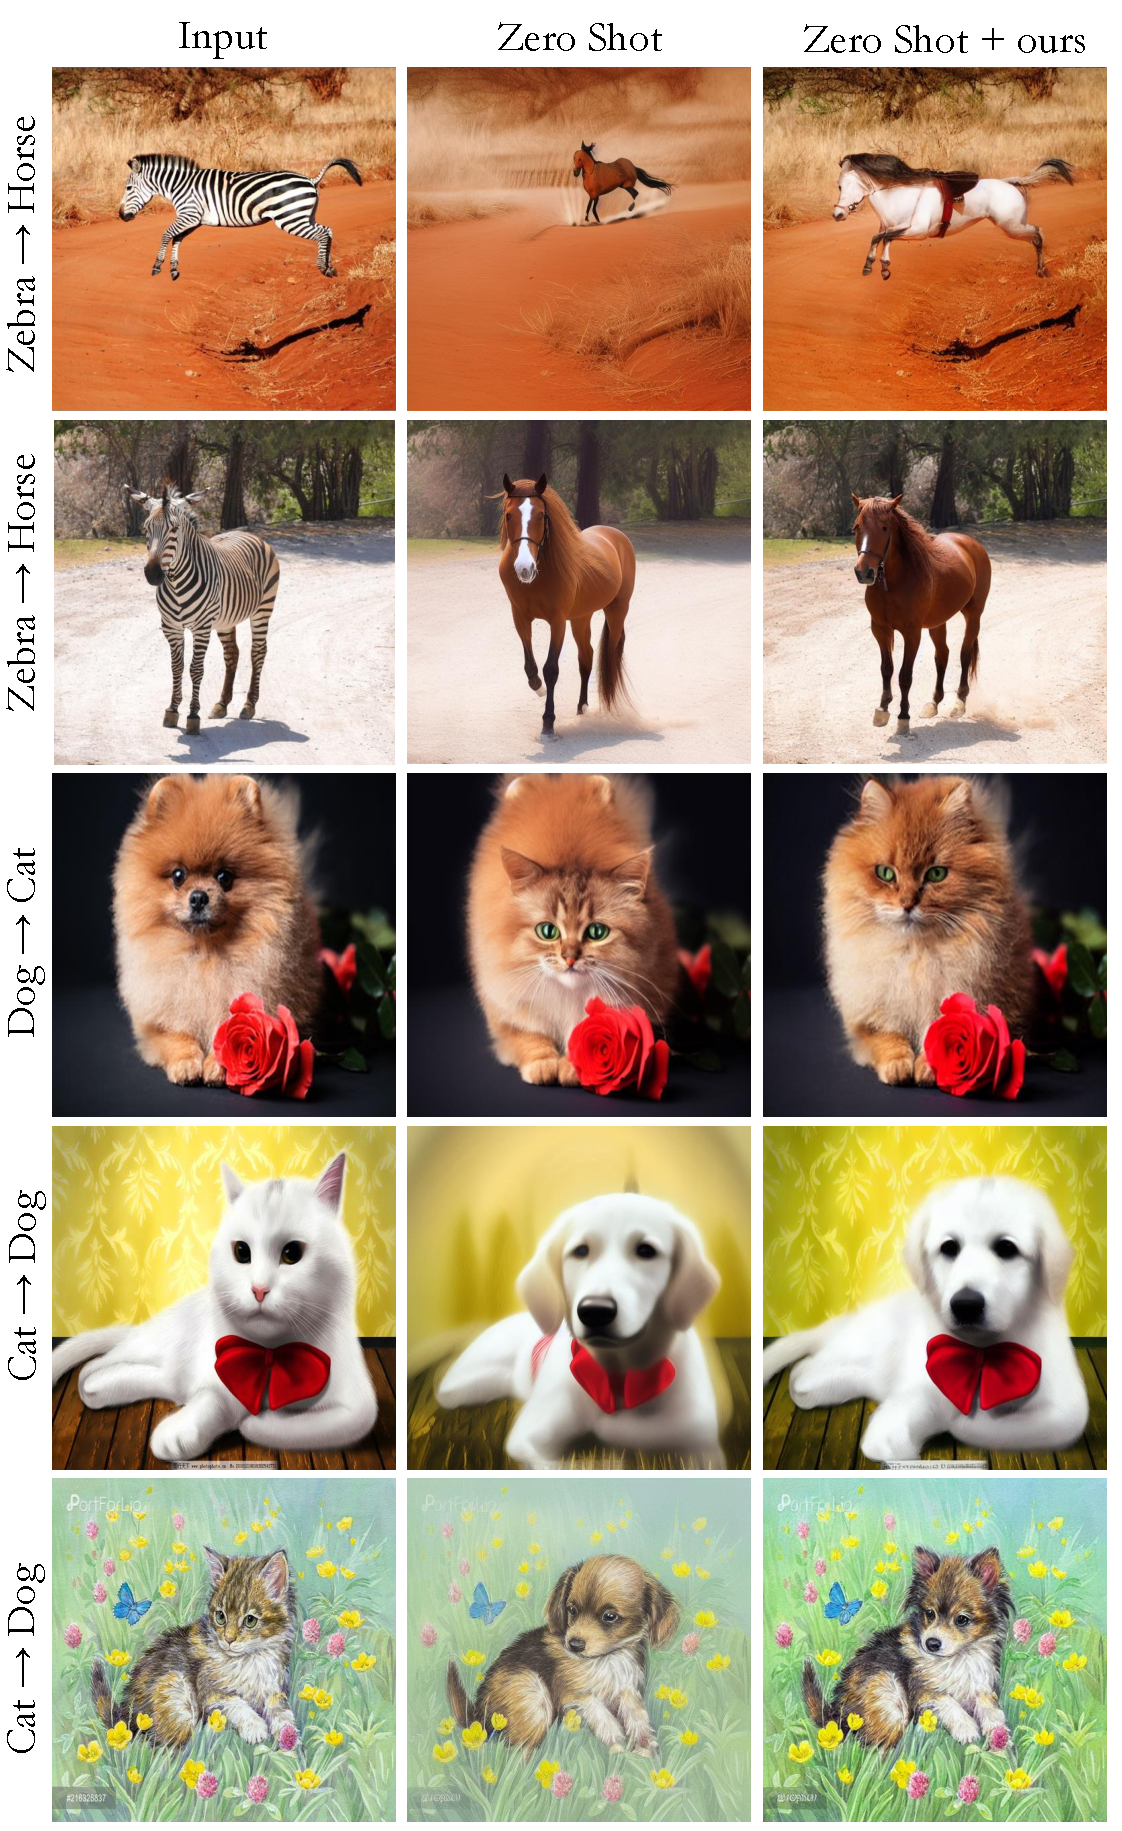
\includegraphics[width=0.96\columnwidth]{ICCV23_submission/figures/zero-shot-results.pdf}
\caption{\textbf{Improving Zero-Shot I2I Translation.} Images generated by Zero Shot I2I suffer from loss of detail. With our inversion, fine textures, like fur and flowers, are retained. 
% Zero-shot results use the default cross-attention guidance weight, 0.1, while the results with our inversion use the cross-attention guidance weight of 0.03. 
Both methods achieve CLIP accuracy of 0.88, however, Zero-Shot method achieves LPIPS score of 0.35 while Zero-Shot with our inversion produces images more similar to the input, and hence, achievs an LPIPS score of 0.27 (for LPIPS lower is better).}
\label{fig:zero-short-qualitative}
% \end{center}
% \vskip -0.2in
\end{figure}
% As seen in Fig.~\ref{fig:clip_lpips}, our inversion achieves a good balance between LPIPS and CLIP. Integrating our inversion into P2P improves their performance in both metrics. Please see more analyses in the Supplementary.
% , while requiring short edit times and supporting diversity among generated outputs.


% In Fig.~\ref{fig:clip_lpips} we show the CLIP-LPIPS losses graph for all methods reported in the paper. In this graph, we show three different parameter configurations for our inversion, for P2P with our inversion, and for CycleDiffusion. As can be seen, our method (by itself or with P2P) achieves the best LPIPS distance for any given level of CLIP similarity.

\vspace{-0.3cm}
\paragraph{Comparisons on the modified Zero-Shot I2IT dataset}
Next, we compare our method to Zero-Shot Image-to-Image Translation (Zero-Shot)~\cite{Parmar23}, which uses DDIM inversion.
This method only translates between several predefined classes. We follow their setting and use $50$ diffusion steps. When using with our inversion, we decrease the hyper-parameter controlling the cross-attention from the default value $0.1$ to $0.03$. As can be seen in Fig.~\ref{fig:zero-short-qualitative}, while Zero-Shot's results comply with the target text, they are typically blurry and miss detail. Integrating our inversion adds back the details from the input image. See more details in the SM.%together with the high value of cross-attention strength disturbing the synthesis process to change to the target prompt.
 % As seen in Tab.~\ref{tab:comparison_table_zero}, integrating our inversion improves the similarity to the input image while keeping the CLIP accuracy high and exhibiting non-negligible diversity among the generated outputs. See more details in the Supplementary.

% \begin{table}
% \centering
% \footnotesize
% \begin{tabular}{| c | c c c c|} 
%  \hline
%  Method & CLIP sim.$\uparrow$ & LPIPS$\downarrow$ & Diversity$\uparrow$ & Time \\[0.5ex]
%  \hline\hline
%  DDIM inv.  & 0.31 & 0.62 & 0.00 & 39\\
%  PnP & 0.31 & 0.36 & 0.00 & 206\\ 
%   CycleDiffusion, \!$\eta\!=\!0.1$ & 0.29 & \bf{0.2} & \bf{0.21} & 40\\ 
%   CycleDiffusion, \!$\eta\!=\!1.0$ & 0.3 & 0.26 & \bf{0.306} & 40\\ 
% P2P & 0.30 & 0.61 & 0.00 & 40\\
%  %\hline
% %\hline
% \bf{P2P+Our}  & 0.31 & \bf{0.25} & 0.11 & 48\\  %[1ex] 
% \bf{Our inv.}  & \bf{0.32} &0.29 & \bf{0.18} & \bf{36}\\
% %\hline
% %\hline
% \hline
% % \bf{Our inv.} & 9 & 36 & 0.32 & 0.24 & ?\\ 
% % \hline
% \end{tabular}
% \caption{Evaluation on modified ImageNet-R-TI2I dataset.}
% \label{tab:comparison_table}
% \end{table}

% \vspace{-0.2cm}

% \begin{table}
% \centering
% \footnotesize
% \begin{tabular}{|c | c c c c|} 
%  \hline
%  Method & CLIP Acc.$\uparrow$ & LPIPS$\downarrow$ & Diversity$\uparrow$ & Time\\
% \hline\hline
% Zero-Shot  & 0.88 & 0.35 & 0.07 &\bf{45}\\ 
% %\hline
% \bf{Zero-Shot+Our} & \bf{0.88} & \bf{0.27} & \bf{0.16} & 46\\  %[1ex] 
% \hline
% % \bf{Our inv.} & 9 & 36 & 0.32 & 0.24 & ?\\ 
% % \hline
% \end{tabular}
% \caption{Evaluation on the modified Zero-Shot I2IT dataset.}
% \label{tab:comparison_table_zero}
% \end{table}


% Lastly, as CycleDiffusion.~\cite{Wu22} also suggests an inversion, we compare this method without any modifications.




% Notice, methods that work well on real images use DDIM inversion with large steps, i.e., $T=1000$ in order to improve performances, as Plug-and-Play~\cite{Narek22} suggest. Reducing the number of steps with our inversion might boost the performance. Unfortunately, this paper does not support this change yet so we could not evaluate over it.

% \subsection{Additional Qualitative Results}
% Diffusion clip
% Null inversion
% cyclediffusion


% For the image manipulation, we use unconditional models trained over Imagenet, based on the guided diffusion code \href{https://github.com/openai/guided-diffusion}{https://github.com/openai/guided-diffusion}. These models were trained with $1000$ steps, and we extract and generate using $T=250$ timesteps.



% is applied over the latent space, on a model trained on LAION \href{}{checkpoint} \inbar{add checkpoint}



% Compare vanilla (using Z) to EDICT
% use ours as a first stage for: p2p, pnp, DIffEdit, Zero-shot Image-to-Image Translation
% - image manipulation: qualitative only, just to show the latent space changes capabilities.

% - text:
% competitive (Quantitiavtive): VQGAN+CLIP, Text2Live, prompt 2 prompt +null,Tali Dekel, DiffEdit (not official), CycleDiffusion, DiffueIT, Zero-shot Image-to-Image Translation.

% competitive (Qualitative): DiffusionCLIP, Imagic?

% datasets: create by ourselves.
% \inbar{AAFQ - "dog"->"cat". DiffueIT, DiffEdit. Tali Dekel show DiffuseIT over her dataset.}

% metric: Lpips, clip (LPIPS-CLIP curve), user study, diversity (mean Lpips between couples), mean over the variance of pixels.

% Should check, divide skip to global changing (background and foreground), foreground changing, style transfer.
